\documentclass{standalone}
\usepackage{tikz}
\begin{document}
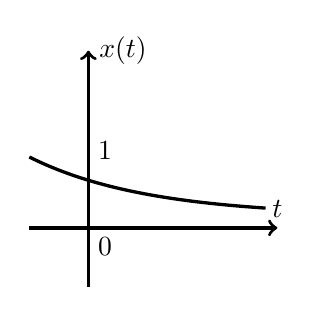
\begin{tikzpicture}[scale=1.5]
    \draw[->,very thick](2,0)--(4.1,0)node[above]{$t$};
        \draw[->,very thick](2.5,-0.5)--(2.5,1.5)node[right]{$x(t)$};
        \draw[-,very thick]plot[smooth, domain=2:4](\x,{1/2*e^(-(\x-2))+0.1});
        \node[above right]at(2.5,0.5){$1$};
        \node[below right]at(2.5,0){$0$};
\end{tikzpicture}
\end{document}